% version 1.01, date 25/02/16, auteur Matthieu Martins-Baltar
\section{Lot 3}
	Le lot 3 devra faire état de cinq fonctionnalités additionnelles. Il devra être impérativement livré au client avant le vendredi 9 décembre 2016. \\
	
	La figure \ref{fonctPrinc} montre l’interaction entre les différentes fonctionnalités à l'aide d'un diagramme de séquence UML.

\begin{figure}[H]
	\begin{center}
	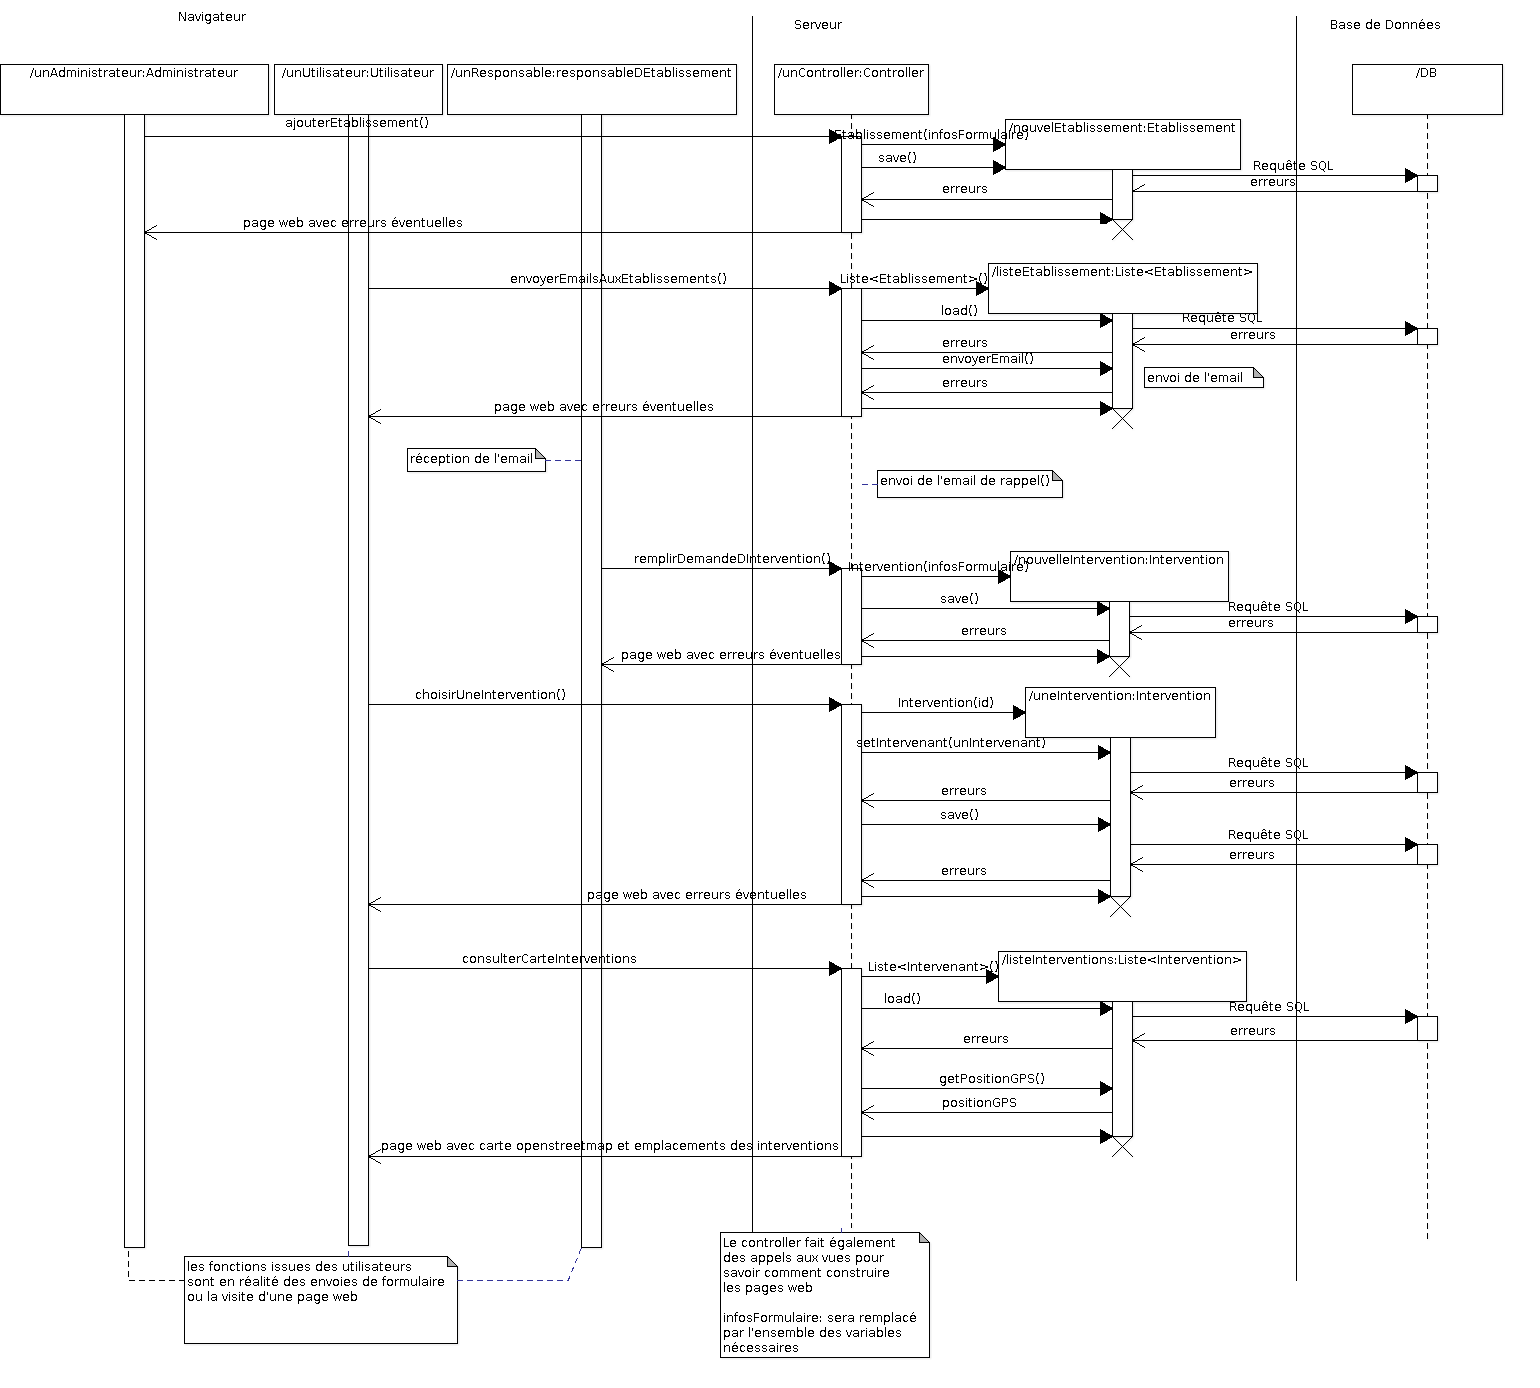
\includegraphics[scale=0.3]{images/fonctionsPrincipales.png}
	\caption{\label{fonctPrinc} Diagramme de séquence représentant les fonctions principales du logiciel}
	\end{center}
\end{figure}

% version 1.00, date 05/11/16, auteur Kafui Atanley
\subsection{Fonctionnalité 8}
La fonctionnalité 7 permettra d’envoyer un e-mail de rappel à l’établissement et au contact
dans l’établissement (si son adresse électronique est différente de celle de l’établissement),
une semaine avant l’intervention.


% version 1.00, date 05/11/16, auteur Kafui Atanley
%L’outil devra faciliter la géolocalisation des établissements, bénévoles et interventions.
%Une carte devra pouvoir être accessible quand l’une des entité possède une adresse et il
%devra être possible de filtrer ces entités en fonction de la distance à une ville ou un point
%géographique particulier à l’aide de liste.
\subsection{Fonctionnalité 9}

La fonctionnalité 9 concerne la géolocalisation des entités possédant une adresse.
Ces entités sont : 
\begin{itemize}
\item les établissements,
\item les interventions quelque soit leur type,
\item les ventes.
\end{itemize}
Une carte devra être affichée dans les fiches détaillées de chaque entité.
La maquette \ref{fonctionnalite9Geolocalisation} présente la fiche descriptive d'une entité. Les fiches descriptives
des entités interventions et ventes devront comporter une carte de manière similaire.
Il devra être possible de filtrer ces entités selon une ville et selon la distance par rapport à une ville.
La maquette \ref{fonctionnalite9Filtre} présente un modèle des filtres attendus sur les entités concernées.

\begin{figure}[H]
	\centering
	\includegraphics[scale=0.4]{images/maquettes/fonctionnalite9Geolocalisation.png}
	 \caption{Maquette~: Géolocalisation dans les fiches descriptives}
	 \label{fonctionnalite9Geolocalisation}
\end{figure}

\begin{figure}[H]
	\centering
	\includegraphics[scale=0.4]{images/maquettes/fonctionnalite9Filtre.png}
	 \caption{Maquette~: Modèle de filtres attendus}
	 \label{fonctionnalite9Filtre}
\end{figure}


% version 1.00, date 05/11/16, auteur Kafui Atanley
\subsection{Fonctionnalité 10}




\newpage
% version 1.00, date 23/02/16, auteur Matthieu Martins-Baltar
\subsection{Contraintes Produits}
Dans cette sous-partie, nous allons décrire les contraintes produits, c'est-à-dire des contraintes ayant trait au système à proprement parler.\\

L'interface de l'application se présentera sous la forme d'une page web qui sera visualisée à partir d'un navigateur. Les navigateurs principaux, Chrome, Firefox, Safari doivent être compatibles et capables d'afficher correctement la page. L'équipe \PIC{} devra spécifier au client les versions de navigateur compatible avec l'application.  Le code de cette page devra répondre aux normes de la W3C. De plus, l'interface devra être \emph{responsive} et utilisable depuis un smartphone. Enfin, le design de l'interface doit permettre une utilisation simple à un utilisateur inexpérimenté.\\

La partie serveur de l'application devra être légère et pouvoir fonctionner sur un serveur de faible dimension. Au niveau départemental se trouvent 8 plaideurs pour près de 1500 établissements. Si l'application devait s'élargir au niveau national, le nombre de plaideurs passeraient à l'ordre de 200 à 300 individus pour près de 50 000 établissements.\\

 
% version 1.00, date 23/02/16, auteur Matthieu Martins-Baltar
\subsection{Contraintes de Réalisation}
Dans cette sous-partie, nous allons lister les contraintes de réalisation, telles que les demandes de documentation ou des contraintes de langage.\\

Il n'y a aucune contrainte de langage de programmation, mais il est à noter qu'il doit s'agir de langages adaptés aux technologies web. Par exemple la partie frontend de notre application ne pourra être qu'en Javascript car il est installé de base avec les navigateurs.\\

La base de donnée utilisera PostgreSQL et PostGIS afin d'intégrer de manière optimale le service OpenStreetMap.\\

Il est demandé une documentation technique à tous les niveaux du projet. Tout d'abord une documentation conceptuelle, une documentation des packages, une documentation détaillée, ainsi que des tests unitaires détaillés et documentés. Cette documentation doit permettre à une future équipe de développement de retravailler sur le projet sans difficulté. Doivent également être documentées, les règles de programmation, les conventions de nommage et les instructions permettant l'installation du logiciel.\\

Enfin, une documentation utilisateur, accompagnée d'une foire aux questions accessible à tous les utilisateurs sera livrée avec le lot2.


